\documentclass{article}

\usepackage{amsmath,amsthm,amssymb,color,latexsym}
\usepackage{geometry}        
\geometry{letterpaper}    
\usepackage{graphicx}
\usepackage{pdfpages}

\author{Andres Alam Sanchez Torres}

\newcommand{\assignmentno}{1}

% Define the custom counters
\newcounter{assignment}
\newcounter{questionpart}
\setcounter{assignment}{0}  % Initial assignment number

% Define a command for section titles
\newcommand{\assignmentpart}[1]{
    \stepcounter{assignment}  % Increment section counter
    \vspace{2em}
    \noindent\textbf{\assignmentno.\arabic{assignment} #1}
    \vspace{1em}
}

% Define custom environment with spacing
\newenvironment{task}{%
    \vspace{2em}
    \refstepcounter{questionpart}%
    \par\noindent\textbf{Question \assignmentno.\arabic{assignment}.\arabic{questionpart}:} \hspace{0.5em}\textit}{%
    \vspace{1em}\\}

\begin{document}
\noindent Advanced Machine Learning\hfill Assignment 1\\
Andres Alam Sanchez Torres \hfill \today

\noindent\hrulefill

\assignmentpart{Dependencies in a Directed Graphical Model}

\begin{center}
  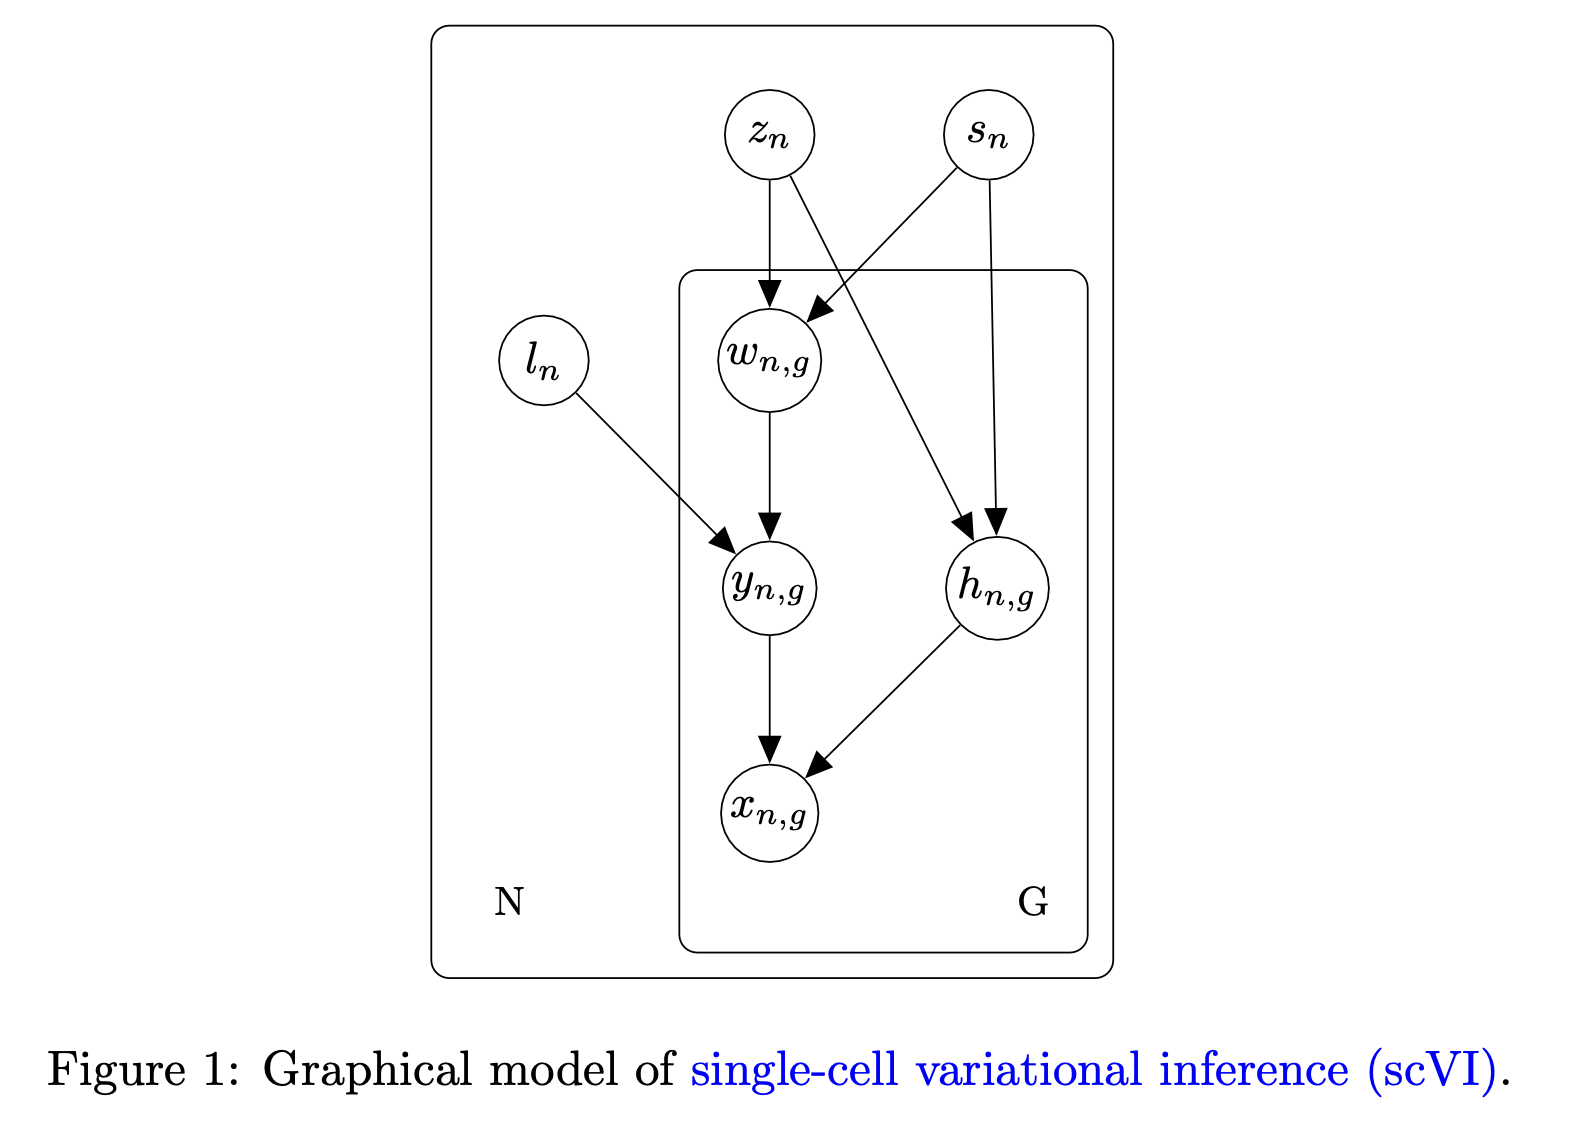
\includegraphics[width=0.8\textwidth]{./figures/dgm1.png}
\end{center}

\begin{task}
  In the graphical model of Figure 1, is \( w_{n, g} \perp w_{n, g + 1} | s_n \)? 
\end{task}

No, there is a non-blocking path $w_{n, g} \leftarrow z_n \rightarrow w_{n, g + 1}$. Since \( s_n \) is not a descendant of \( z_n \), the nodes are not d-separated by \( s_n \), and thus, not conditionally independent.
\begin{task}
  In the graphical model of Figure 1, is \( l_n \perp w_{n, g} | x_{n, g} \)? 
\end{task}
No, there is a path \( l_n  \rightarrow y_{n, g} \leftarrow w_{n, g}\) which is not a d-separation since \( x_{n, g} \) is a descendant of \( y_{n, g} \).

\begin{task}
  In the graphical model of Figure 1, is \( z_{n} \perp x_{n, g} | w_{n, g}, h_{n, g} \)? 
\end{task}
Yes.


\begin{center}
  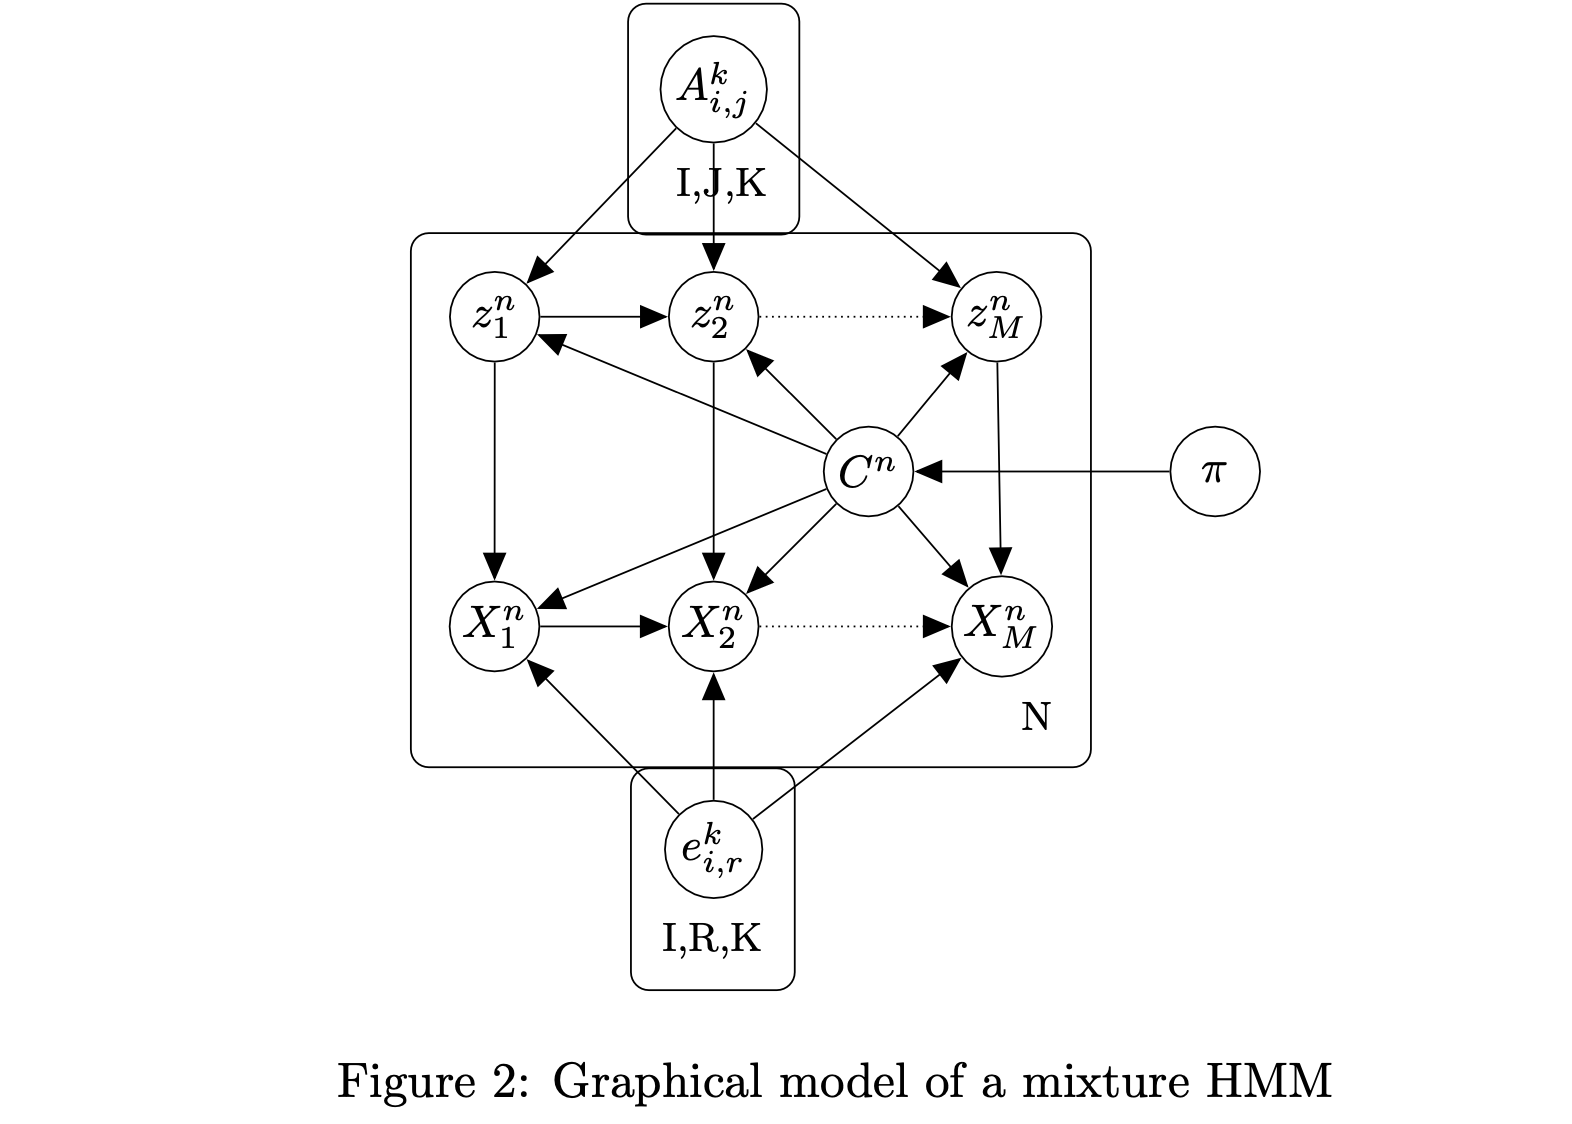
\includegraphics[width=0.8\textwidth]{./figures/dgm2.png}
\end{center}

\begin{task}
  In the graphical model of Figure 2, is \( z_{1}^{n}  \perp z^n_M | C_n, A^{1:K}_{1:I, 1:J} \)? 
\end{task}
No, we can note that there exists a path for any pair \( z_{a}^n, z_b^n \) such that \( a,b \in [1, M]\), consisting on a chain of \( z_m^n \) nodes. These such paths do not include d-separations, thus  
the nodes are not conditionally independent.

\begin{task}
  In the graphical model of Figure 2, is \( X_1^n  \perp X_M^n | X_2^n, C^n \)? 
\end{task}
No, for any \( M > 2 \), we can build a path in the form \( X_1^n \leftarrow e_{i,r}^k \rightarrow X_M^n \), which is not blocked by \( X_2^n, C^n \).

\begin{task}
  In the graphical model of Figure 2, is \( C^n \perp C^{n + 1} | z_{1:M}^n, X^n_{1:M} \)? 
\end{task}
No, there exists the dependency \( C^n \leftarrow \pi \rightarrow C^{n + 1}\), not conditioned by either. 


\assignmentpart{CAVI}
\begin{task}
  Find ML estimates of the variables $\mu$ and $\tau$. (1 points)
\end{task}


We first state the likelihood function by the assumption of i.i.d. observations. The joint probability of observing $\mathbf{X} = \{x_1,...,x_N\}$ is:

\begin{align*}
p(\mathbf{X}|\mu,\tau) &= \prod_{n=1}^N p(x_n|\mu,\tau) \\
&= \prod_{n=1}^N \mathcal{N}(x_n|\mu,\tau^{-1}) \\
&= \prod_{n=1}^N \sqrt{\frac{\tau}{2\pi}} \exp\left(-\frac{\tau}{2}(x_n-\mu)^2\right)
\end{align*}
The Maximum Likelihood estimation problem can then be formulated as:

\begin{align*}
(\hat{\mu}_{\text{ML}}, \hat{\tau}_{\text{ML}}) &= \arg\max_{\mu , \tau } p(\mathbf{X}|\mu,\tau) \\
&= \arg\max_{\mu, \tau} \log  \left(\prod_{n = 1}^N p(x_n | \mu, \tau) \right) \\ 
&= \arg\max_{\mu, \tau} \underbrace{\sum_{n = 1}^n \log   p(x_n | \mu, \tau) }_{=: \mathcal{L}}
\end{align*}

\begin{align*}
\mathcal{L} &= \sum_{n = 1}^N \log \left( \sqrt{\frac{\tau}{2\pi}} \exp\left(-\frac{\tau}{2}(x_n-\mu)^2\right) \right) \\
&= \sum_{n = 1}^N -\frac{\tau}{2}(x_n-\mu)^2 + N \log \sqrt{\frac{\tau}{2\pi}} \\
&= \sum_{n = 1}^N -\frac{\tau}{2}(x_n-\mu)^2 + \frac{N}{2} \log \tau - \frac{N}{2} \log (2 \pi) \\
\end{align*}

This is maximized when the partial derivatives with respect to $\mu$ and $\tau$ are zero. We then have:

\begin{align*}
\frac{\partial \mathcal{L}}{\partial \mu} &= \tau\sum_{n=1}^N(x_n-\mu) \\ 
\frac{\partial \mathcal{L}}{\partial \tau} &= \frac{N}{2\tau} - \frac{1}{2}\sum_{n=1}^N(x_n-\mu)^2 
\end{align*}

Then, 
\begin{align*}
\hat{\mu}_{\text{ML}} &= \frac{1}{N}\sum_{n=1}^N x_n  \\
\hat{\tau}_{\text{ML}} &= \frac{N}{\sum_{n=1}^N(x_n-\hat{\mu}_{\text{ML}})^2} 
\end{align*}


\begin{task}
  What is the exact posterior?
\end{task}

  The posterior distribution \(p(\mu, \tau \mid \mathbf{X})\) can be derived using Bayes' theorem:
  \[
  p(\mu, \tau \mid \mathbf{X}) \propto p(\mathbf{X} \mid \mu, \tau) p(\mu \mid \tau) p(\tau).
  \]
  
  Given
  \[
  p(\mathbf{X} \mid \mu, \tau) = \left(\frac{\tau}{2\pi}\right)^{N/2} \exp\left(-\frac{\tau}{2} \sum_{n=1}^N (x_n - \mu)^2\right).
  \]
  
  \[
  p(\mu \mid \tau) = \mathcal{N}(\mu \mid \mu_0, (\lambda_0 \tau)^{-1}) = \sqrt{\frac{\lambda_0 \tau}{2\pi}} \exp\left(-\frac{\lambda_0 \tau}{2} (\mu - \mu_0)^2\right).
  \]
  
  \[
  p(\tau) = \mathrm{Gamma}(\tau \mid a_0, b_0) = \frac{b_0^{a_0}}{\Gamma(a_0)} \tau^{a_0 - 1} \exp(-b_0 \tau).
  \]
  
  and plugging them into Bayes' theorem, the joint posterior is proportional to (isolating the terms involving \(\mu\) and \(\tau\)):
  \begin{align*}
    p(\mu, \tau \mid \mathbf{X}) &\propto \tau^{\frac{N}{2}} \exp\left(-\frac{\tau}{2} \sum_{n=1}^N (x_n - \mu)^2\right) \cdot \sqrt{\lambda_0 \tau} \exp\left(-\frac{\lambda_0 \tau}{2} (\mu - \mu_0)^2\right) \cdot \tau^{a_0 - 1} \exp(-b_0 \tau)\\
     &\propto \tau^{\frac{N}{2} + a_0 - 1 + \frac{1}{2}}  \exp\left( -\frac{\tau}{2} \sum_{n = 1}^N(x_n - \mu)^2 - \frac{\lambda_0 \tau}{2} (\mu - \mu_0)^2 -b_0 \tau \right) \\ 
     &\propto \tau^{\frac{N}{2} + a_0 - \frac{1}{2}}  \exp\left( -\frac{\tau}{2} \left( \sum_{n = 1}^N(x_n - \mu)^2 + \lambda_0 (\mu - \mu_0)^2 \right) - b_0 \tau \right). 
  \end{align*}
% 
%

Completing the square for the expression
\[
\sum_{n=1}^N (x_n - \mu)^2 + \lambda_0 (\mu - \mu_0)^2 = (\lambda_0 + N)(\mu - \mu_N)^2 + C,
\]
where:
\[
\mu_N = \frac{\lambda_0 \mu_0 + N \bar{x}}{\lambda_0 + N}, \quad
C = \lambda_0 \mu_0^2 + \sum_{n=1}^N x_n^2 - (\lambda_0 + N)\mu_N^2.
\]

Then,
\begin{align*}
  p(\mu, \tau \mid D) &\propto \tau^{\frac{N}{2} + a_0 - \frac{1}{2}}  \exp\left( -\frac{\tau}{2} \left( (\lambda_0 + N) (\mu - \mu_N)^2 + C \right) - b_0 \tau \right) \\ 
  &\propto \tau^{a_0 + \frac{N}{2} - \frac{1}{2}}  \exp\left(-\tau \left(b_0 + \frac{C}{2}\right)\right) \cdot \exp\left(-\frac{\tau (\lambda_0 + N)}{2} (\mu - \mu_N)^2\right)\\
  &\propto \underbrace{\tau^{a_0 + \frac{N}{2} - \frac{1}{2}}  \exp\left(-\tau \left(b_0 + \frac{C}{2}\right)\right)}_{\mathrm{Gamma}} \cdot \underbrace{\exp\left(-\frac{\tau (\lambda_0 + N)}{2} (\mu - \mu_N)^2\right)}_{Gaussian}.
\end{align*}

  
  The posterior is thus separable into the following components:
    \[
   p(\mu \mid \tau, D) = \mathcal{N}\left(\mu \mid \mu_N, (\lambda_N \tau)^{-1}\right), \quad \text{where } \lambda_N = \lambda_0 + N.
  \]
   \[
  p(\tau \mid D) = \mathrm{Gamma}\left(\tau \mid a_0 + \frac{N+1}{2}, \, b_0 + \frac{1}{2} \left(\sum_{n=1}^N (x_n - \bar{x})^2 + \frac{\lambda_0 N}{\lambda_0 + N} (\bar{x} - \mu_0)^2\right)\right).
  \]
  
  Combining these results, the exact posterior distribution is:
  \[
    p(\mu, \tau \mid D) \propto \mathrm{Gamma}\left(\tau \mid a_0 + \frac{N+1}{2}, \, b_0 + \frac{1}{2} \left(\sum_{n=1}^N (x_n - \bar{x})^2 + \frac{\lambda_0 N}{\lambda_0 + N} (\bar{x} - \mu_0)^2\right)\right) \cdot \mathcal{N}\left(\mu \mid \mu_N, (\lambda_N \tau)^{-1}\right).
  \]

  \begin{task}
    Implement the VI algorithm for the variational distribution in Equation (10.24) in Bishop. Run the VI algorithm on the datasets. Plot the ELBO results. Compare
  the inferred variational distribution with the exact posterior and the ML estimate. Visualize the
  results and discuss your findings. 
  \end{task}

  \includepdf[pages=-]{export.pdf}
  

\end{document}

